\chapter{信号処理技術の画像データへの応用}

本章では,離散フーリエ変換の画像データへの応用について紹介し,
また信号処理におけるフィルタ処理の一部を画像データへ活用する.
なお,実装する環境を以下に示す.


\begin{itemize}
  \item OS: Windows10
  \item プログラム言語: Python 3.6
  \item ライブラリ
  \begin{itemize}
    \item NumPy: 数値計算ライブラリ
    \item OpenCV: 画像処理ライブラリ
    \item MatPlotLib: 画像出力ライブラリ
  \end{itemize}
\end{itemize}

\section{離散フーリエ変換の画像データへの応用}

これまでの離散フーリエ変換(式(\ref{eq:dft}))は時間空間の1次元離散データにおける
周波数成分を抽出し,離散逆フーリエ変換(式(\ref{eq:idft}))を用いて
時間領域のデータへ復元していた.
この1次元データ上での離散フーリエ変換を画像データへ応用するには,画像を2次元の
時間空間における離散データ$f(x, y)$とみなし,$x, y$それぞれの方向に対して
離散フーリエ変換(式(\ref{eq:dft_2d}))することで,2次元の周波数成分$F(u, v)$を算出できる.
\begin{align}
  F(u, v) = \sum_{x = 0}^{M-1} \sum_{y = 0}^{N-1} f(x, y) e ^ {- 2 \pi \left(\frac{ux}{M} + \frac{vy}{N} \right) j} \label{eq:dft_2d}
\end{align}
\autoref{fig:input_example},\autoref{fig:dft_example}
に画像データへ離散フーリエ変換を行った例を示す.
\autoref{fig:input_example}は入力画像であり,
\autoref{fig:dft_example}は入力画像の周波数領域である.
この図では,図の中心に近い領域は低周波成分を示し,中心から離れていくほど高周波成分を示している.
\autoref{Fig:dft_example}に対して信号処理にて用いられているバンドパスフィルタを
用いることで信号処理技術でのフィルタ処理を画像データに応用できる.

離散フーリエ逆変換も式(\ref{eq:dft_2d})と同様に$(u, v)$それぞれの方向に対して
逆変換を行うことで\autoref{fig:dft_example}から元の画像へ復元できる(式(\ref{eq:idft_2d})).
\begin{align}
  f(x, y) = \frac{1}{MN} \sum_{u = 0}^{M-1} \sum_{v = 0}^{N-1} F(u, v) e ^ {2 \pi \left(\frac{ux}{M} + \frac{vy}{N} \right) j} \label{eq:idft_2d}
\end{align}
\iffigure
\begin{figure}[h]
  \centering
  \begin{minipage}{.45\hsize}
    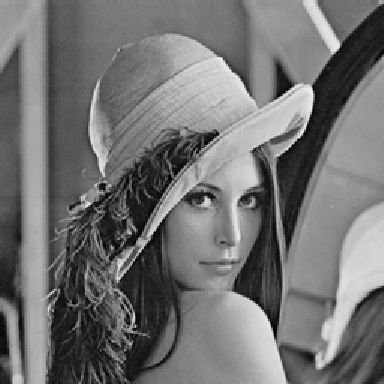
\includegraphics[clip, width=\textwidth]{figure/Lenna.pdf}
    \caption{入力画像}
    \label{fig:input_example}
  \end{minipage}
  \begin{minipage}{.45\hsize}
    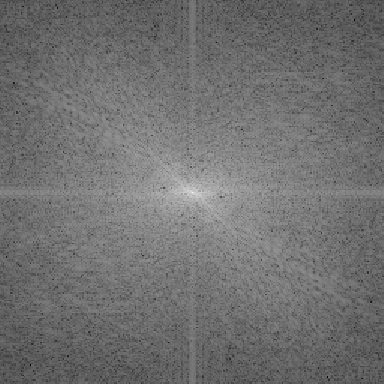
\includegraphics[clip, width=\textwidth]{figure/Lenna_dft.pdf}
    \caption{入力画像の周波数成分}
    \label{fig:dft_example}
  \end{minipage}
\end{figure}
\fi

\section{ハイパスフィルタによる画像処理}

\autoref{code:high_pass}に,画像に対してハイパスフィルタを行う$\mathsf{high\_pass\_img}()$関数を示す.
\autoref{code:high_pass}では,入力された画像から離散フーリエ変換を用いて周波数成分を抽出し,
$x, y$それぞれのカットオフ周波数より低い周波数領域に0を代入したのちに離散フーリエ逆変換
を用いて画像へと復元する.ただし,処理時間の都合上,離散フーリエ変換,逆変換はNumPy
ライブラリにて実装されている高速フーリエ変換を用いる.
\lstinputlisting[caption=画像へのハイパスフィルタを行う$\mathsf{high\_pass\_img}()$関数, label={code:high_pass}]{script/show_high_pass.py}

\autoref{fig:high_input}に入力画像,
\autoref{fig:high_pass_dft}に\autoref{fig:dft_high}に対してハイパスフィルタで
処理した後の周波数成分,
\autoref{fig:high_pass_idft}に復元した出力画像を示す.
\autoref{fig:high_pass_idft}より,画像内の顔の輪郭や髪の毛などといったよなピクセル間の
温度差の激しい部分,すなわちエッジが抽出できており,
逆に帽子の模様や鏡の縁のようなピクセル間の温度差が類似している部分が除去されている.
このことから,画像データに対してハイパスフィルタを用いることにより
画像のエッジ抽出として活用することができる.

\iffigure
\begin{figure}[h]
  \centering
  \begin{minipage}{.25\hsize}
    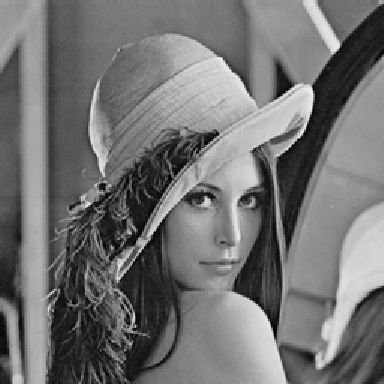
\includegraphics[clip, width=\textwidth]{figure/Lenna.pdf}
    \caption{入力画像}
    \label{fig:high_input}
  \end{minipage}
  \begin{minipage}{.25\hsize}
    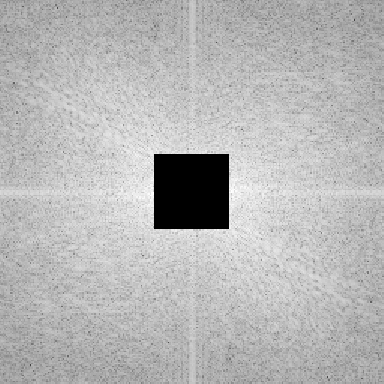
\includegraphics[clip, width=\textwidth]{figure/high_pass_dft_2d.pdf}
    \caption{ハイパスフィルタによる抽出}
    \label{fig:high_pass_dft}
  \end{minipage}
  \begin{minipage}{.25\hsize}
    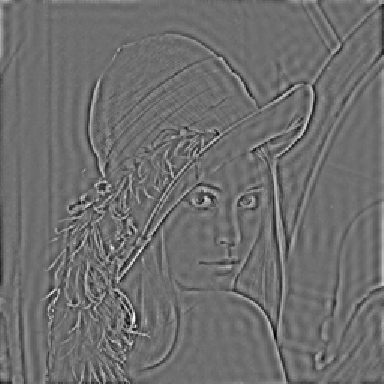
\includegraphics[clip, width=\textwidth]{figure/high_pass_idft_2d.pdf}
    \caption{処理後の画像}
    \label{fig:high_pass_idft}
  \end{minipage}
\end{figure}
\fi

\section{ローパスフィルタのによる画像処理}

\autoref{code:low_pass}に,画像に対してローパスフィルタを行う$\mathsf{low\_pass\_img}()$関数を示す.
\autoref{code:low_pass}では,\autoref{code:low_pass}と同様に
入力された画像の周波数成分を抽出し, $x, y$それぞれのカットオフ周波数より高い周波数領域
に0を代入したのちに逆変換を用いて画像へと復元する.
\lstinputlisting[caption=画像へのローパスフィルタを行う$\mathsf{low\_pass\_img}()$関数, label={code:low_pass}]{script/show_low_pass.py}

\autoref{fig:low_input}に入力画像,
\autoref{fig:low_pass_dft}に\autoref{fig:dft_low}に対してローパスフィルタで
処理した後の周波数成分,
\autoref{fig:low_pass_idft}に復元した出力画像を示す.
\autoref{fig:low_pass_idft}と\autoref{fig:low_input}を比較すると,
画像内の輪郭がぼやけており鮮明さが失われていることがわかる.
このことから,画像データに対してローパスフィルタを用いると画像に対してぼかしをかける
処理として活用することができる.

\iffigure
\begin{figure}[h]
  \centering
  \begin{minipage}{.25\hsize}
    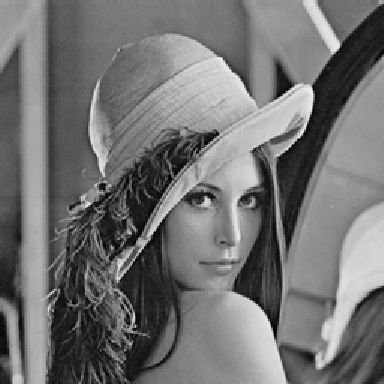
\includegraphics[clip, width=\textwidth]{figure/Lenna.pdf}
    \caption{入力画像}
    \label{fig:low_input}
  \end{minipage}
  \begin{minipage}{.25\hsize}
    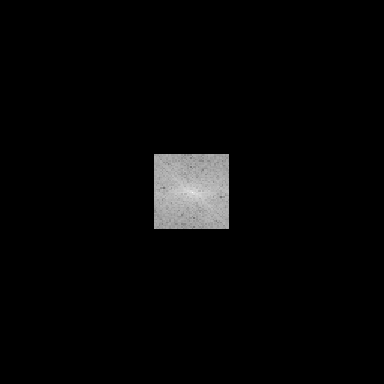
\includegraphics[clip, width=\textwidth]{figure/low_pass_dft_2d.pdf}
    \caption{ローパスフィルタによる抽出}
    \label{fig:low_pass_dft}
  \end{minipage}
  \begin{minipage}{.25\hsize}
    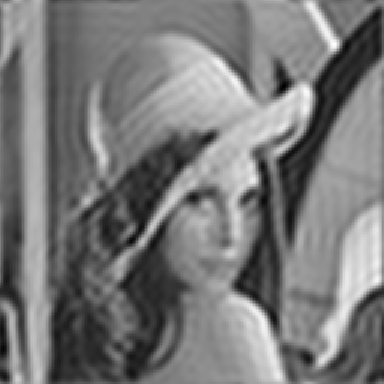
\includegraphics[clip, width=\textwidth]{figure/low_pass_idft_2d.pdf}
    \caption{処理後の画像}
    \label{fig:low_pass_idft}
  \end{minipage}
\end{figure}
\fi

